
% This LaTeX was auto-generated from an M-file by MATLAB.
% To make changes, update the M-file and republish this document.

\documentclass{article}
\usepackage{graphicx}
\usepackage{color}

\sloppy
\definecolor{lightgray}{gray}{0.5}
\setlength{\parindent}{10pt}
\usepackage[margin=1in]{geometry}

\begin{document}

\title{Dynamical Adaptation in ORNs}
\author{Srinivas Gorur-Shandilya}
\maketitle

    
    
\section*{Why is the Slope not 1?}

\begin{par}
The best fit line to the prediction from a linear filter and the data should be 1. But it isn't.
\end{par} \vspace{1em}
\begin{par}
First we make an Gaussian noise input and create an exponential filter, and make the output by convolving the filter with the input.
\end{par} \vspace{1em}
\begin{par}
We can now reconstruct the filter:
\end{par} \vspace{1em}

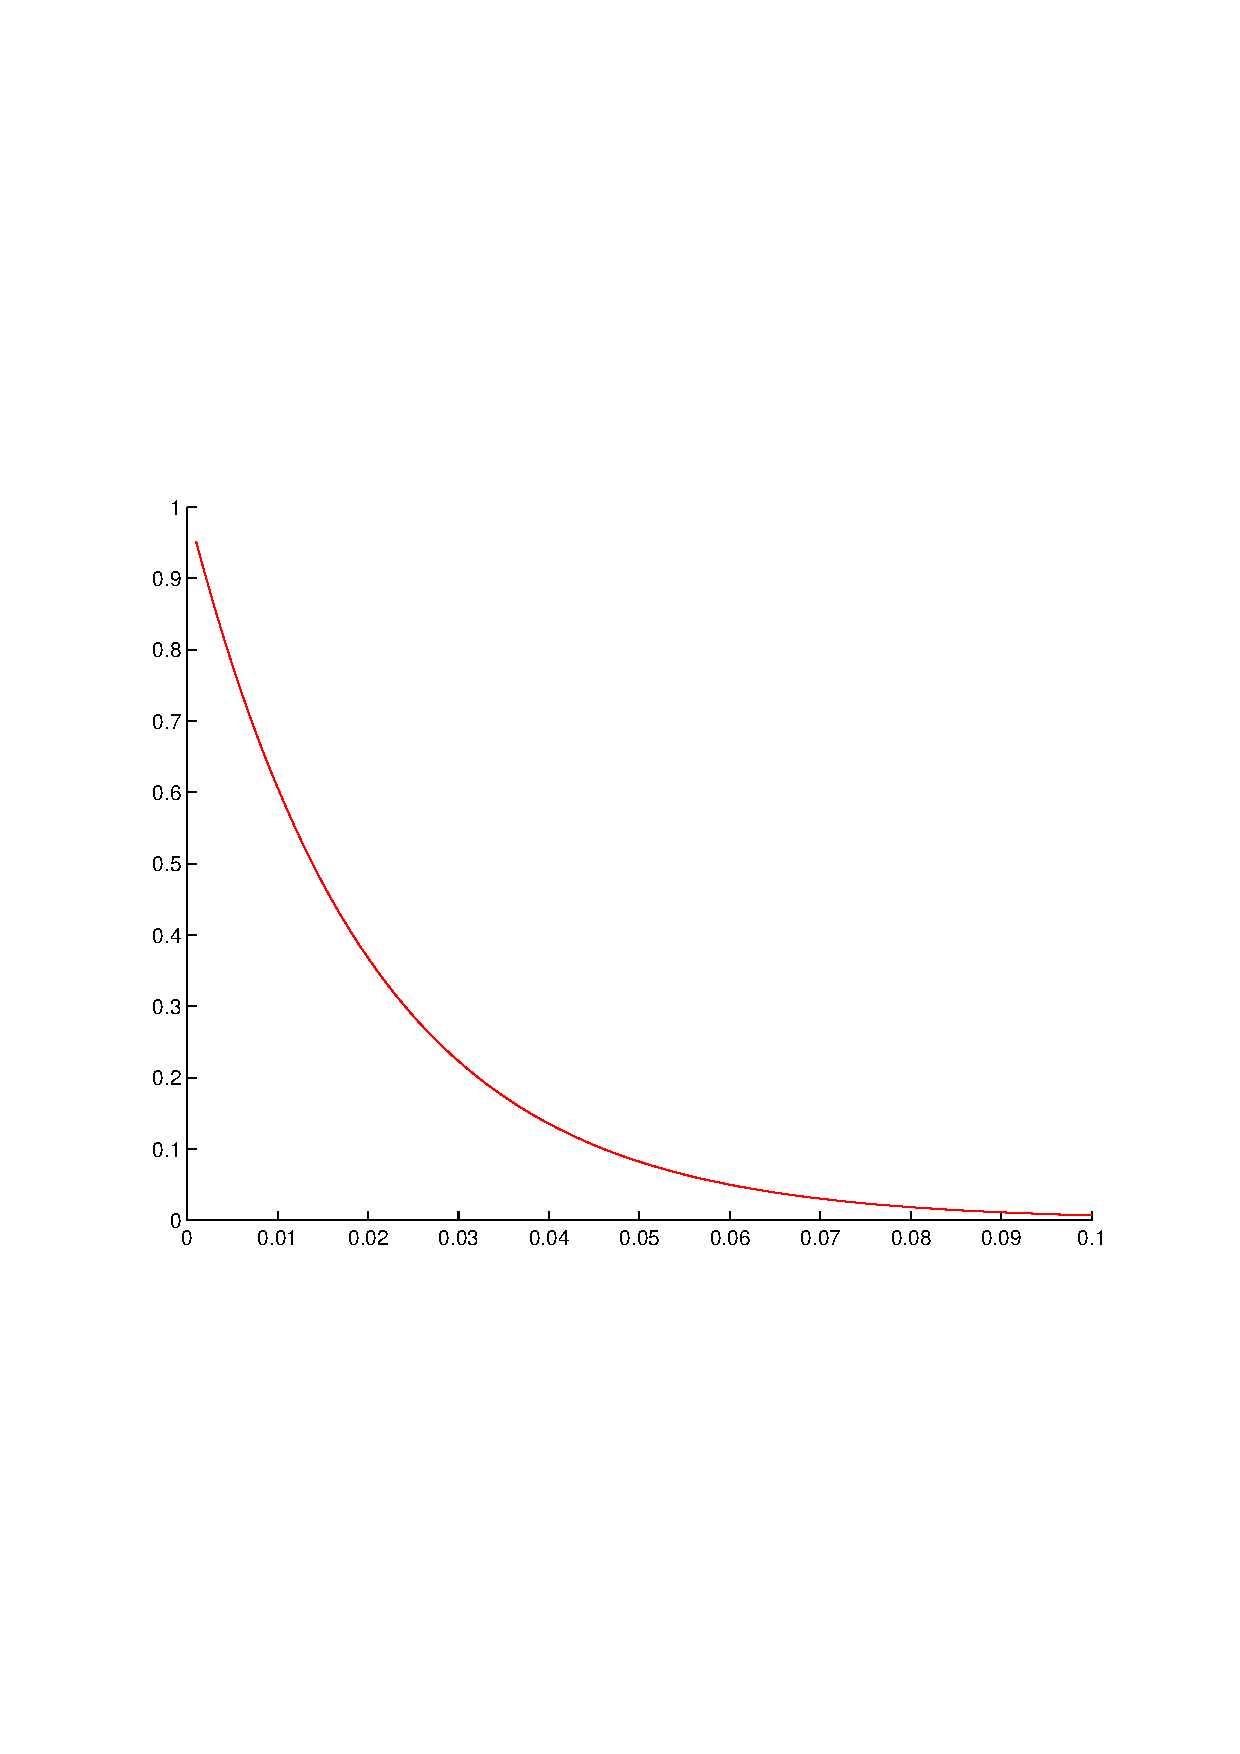
\includegraphics [width=\textwidth]{SlopeProblem_01.pdf}
\begin{par}
and the slope of best fit is:
\end{par} \vspace{1em}

        \color{lightgray} \begin{verbatim}    1.0000

\end{verbatim} \color{black}
    \begin{par}
Now, we add some Gaussian noise to the output.
\end{par} \vspace{1em}

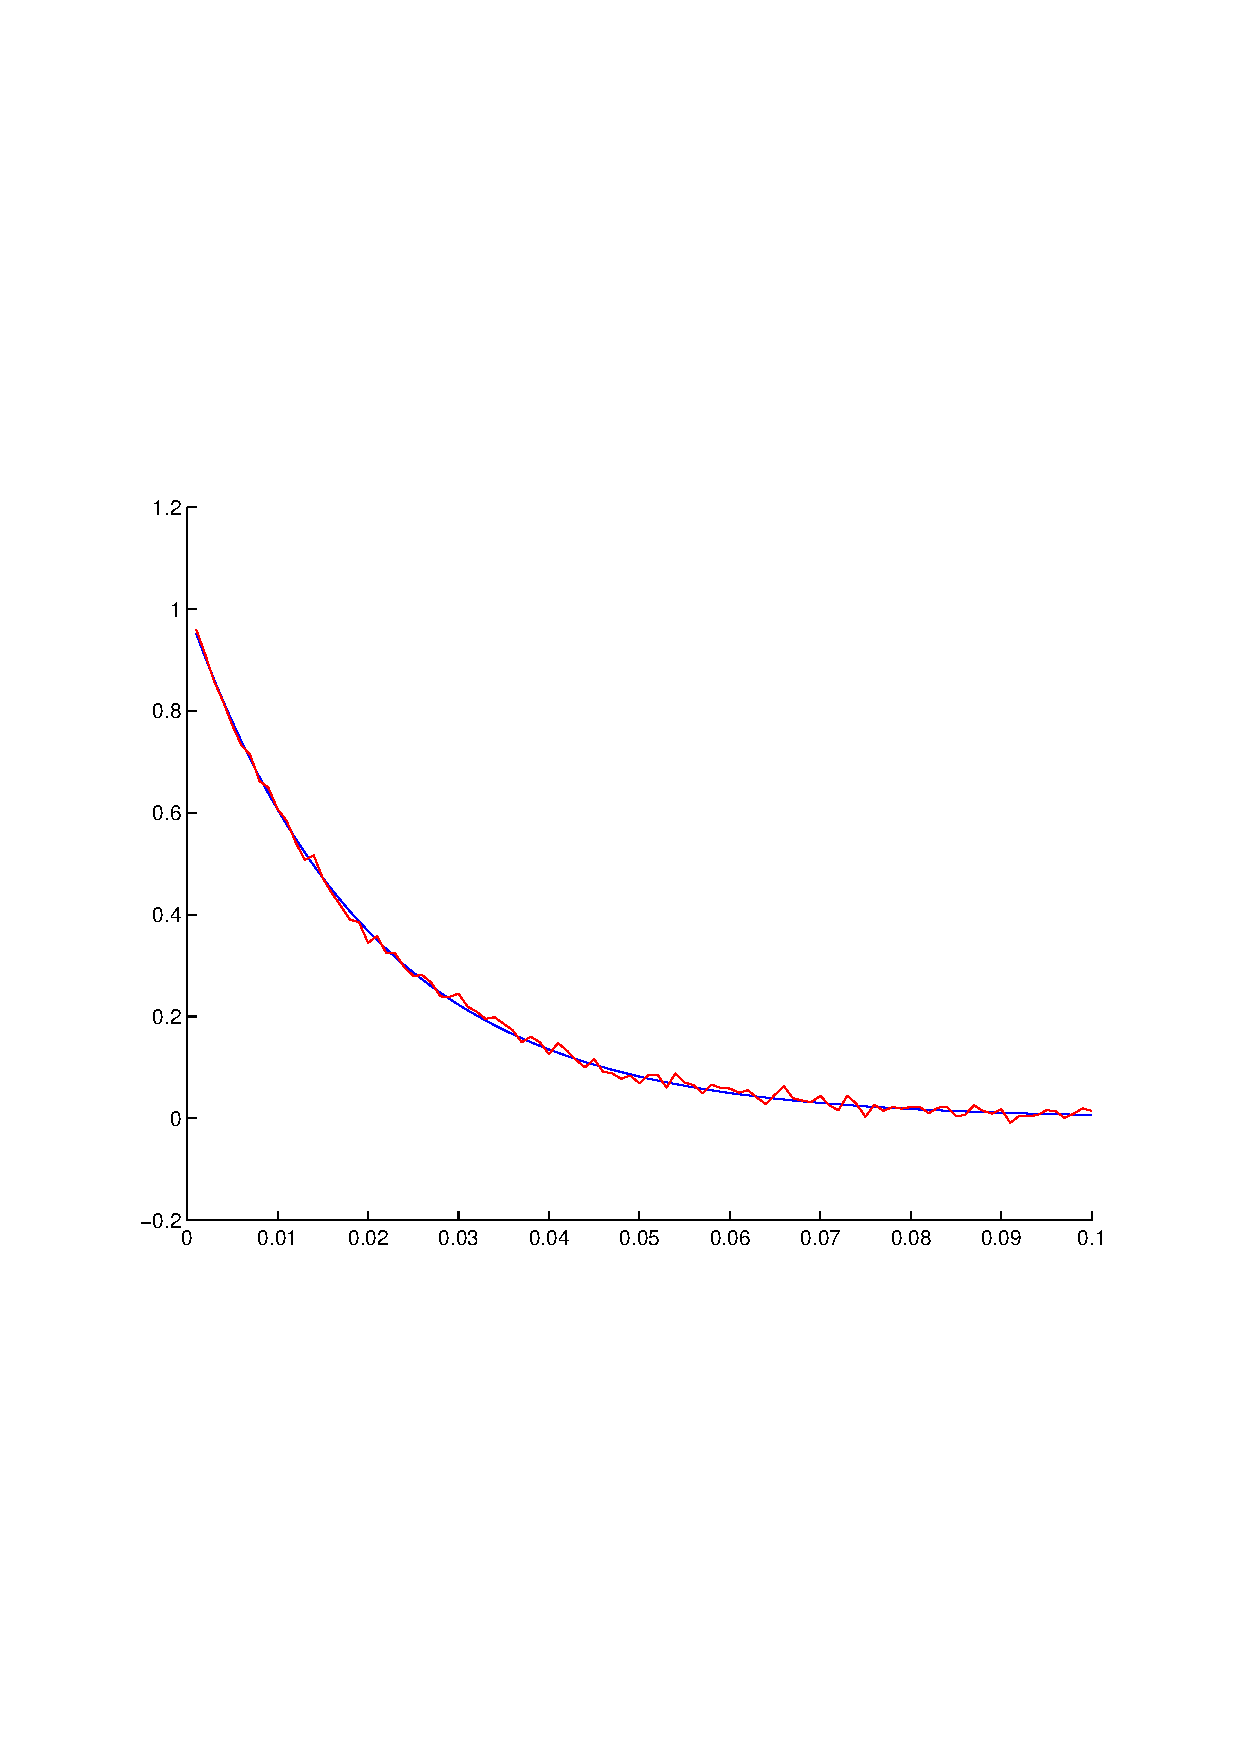
\includegraphics [width=\textwidth]{SlopeProblem_02.pdf}
\begin{par}
and the slope of best fit is:
\end{par} \vspace{1em}

        \color{lightgray} \begin{verbatim}    1.0003

\end{verbatim} \color{black}
    \begin{par}
but if we calculate the inverse slope, it is not the inverse of the slope:
\end{par} \vspace{1em}

        \color{lightgray} \begin{verbatim}    0.9033

\end{verbatim} \color{black}
    \begin{par}
Very strange, but that concludes the slope problem.
\end{par} \vspace{1em}



\end{document}
    
